\chapter{Lecture 26}
\lhead{March 23, 2015}
\chead{21-366 Lambda Calculus Lecture 26}
\rhead{Brian Jacobs}
\pagestyle{fancy}

\section{Head Normal Form}
Recall: The general form of a term:
\begin{equation*}
  \l x_1\ldots x_n.x_1X_1\ldots X_m
\end{equation*}
with $n \geq 0, m \geq 0$ and $i \in \mathbb{N}$. This is called head normal form. The head variable is $x_i$.
\begin{equation*}
  \l x_1\ldots x_n(\underbrace{(\l x X_0)X_1}_{\hbox{head redex}}\ldots X_m)
\end{equation*}
with $n \geq 0$ and $m \geq 1$.\\

A term $X$ is said to have a head normal form $Y$ if $X =_\beta Y$ and $Y$ is in head normal form. This is highly nonunique.\\

Suppose that $Y$ is a head normal form, and $Y \twoheadrightarrow_\beta Z$. THen we know that $Z$ is also a normal form. It has the same lambda prefix $(n)$ and the same head variable $(i)$, and the same number of components $m$. Therefore if $X =_\beta Y$, $Y$ is in head normal form by church rosser.
\begin{equation*}
  X \twoheadrightarrow_\beta Z \twoheadleftarrow Y
\end{equation*}
Therefore, $X \twoheadrightarrow_\beta$ to a head normal form.\\

But $X \twoheadrightarrow_\beta Z$, where $Z$ is in head noraml form. In the head reduction part, $\l y_1,\ldots,y_r((\l yY_0)Y_1\ldots Y_s)$. $X \twoheadrightarrow_\beta W \twoheadrightarrow_\beta Z$.\\

\textbf{Theorem:} $X$ has a head normal form if and only if the head reduction sequence beginning with $X$ terminates.\\

\section{Solvability}
\textbf{Definition:} $X$ (a closed term) is said to be solvable if there exists terms $N_1\ldots N_n$ such that $XN_1\ldots N_n =_\beta I$.

\begin{eqnarray*}
  XN_1\ldots N_nK &=& K\\
  XN_1\ldots N_n &=& K\\
  XN_1\ldots N_n II &=& I\\
\end{eqnarray*}

\textbf{Theorem (Wadsworth):} A closed term $M$ is solvable if and only if $M$ has a head normal form.\\

% Note: make all the x_n.x_1 into x_n.x_i
\textbf{Proof:} $M$ has a head normal form $M \twoheadrightarrow_\beta \l x_1\ldots x_n . x_i X_1\ldots X_m$. Then
\begin{equation*}
  M\underbrace{K_*^m\ldots K_*^m}_{\hbox{$m$ times}} \twoheadrightarrow_\beta (\l x_1 \ldots x_n(x_1X_1\ldots X_m))K_*^m\ldots K_*^m \twoheadrightarrow_\beta K_*^m ([K_*^m/x_1,\ldots,K_*^m/x_n])\ldots \twoheadrightarrow_\beta I
\end{equation*}
Conversely, suppose that $M$ is solvable. $M N_1\ldots N_k  \twoheadrightarrow_{\hbox{head reduction }\beta} I$. We cannot reduce any subterms in such a way that $M$ is not in the head position.\\

\textbf{Remark:} $M$ is solvable if and only if there exists a term $F$ such that $FM = K_*$ and for some other term $N$, $FN =_\beta K$.\\

\textbf{Proof:} $M$ is solvable just like before. $F = \l u\ldots u K_*^m\ldots K_*^mFM \twoheadrightarrow_\beta K_*$. $FM = K_*$ and $FN = K$. We need two new variables $x,y$ so that $FMxy =_\beta Y$. $y$ is normal, so there is a head reduction $FMxy \twoheadrightarrow_\beta y$. $MW_1\ldots W_k \twoheadrightarrow_\beta y$.\\

Why does this prove that $M$ has a head normal form? Just put in $I$ for $x$ and $I$ for $y$ and you get $M([I/x,I/y]W_1)\ldots([I/x,I/y]W_k) \twoheadrightarrow_\beta I$.

\subsection{Properties of Unsolvable Terms}
Consider the following procedure on the possibly open term $X$. Perform the head reduction sequence. Either it does not terminate, in which case we have an open term with no head normal form. We call this $\bot$, or bottom. The option is that we get $\l x_1\ldots x_n.x_i$ We break $x_i$ into $X_1\ldots X_m$ and repeat in parallel, creating a finitely branching tree.
\begin{center}
  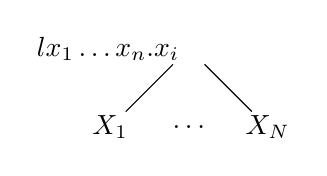
\begin{tikzpicture}
    \draw (0,0) node[anchor=east] {$\l x_1\ldots x_n.x_i$};
    \draw (-0.2,-0.2) -- (-0.8,-0.8);
    \draw (0.2,-0.2) -- (0.8,-0.8);
    \draw (-1,-1) node {$X_1$};
    \draw (0,-1) node {$\ldots$};
    \draw (1,-1) node {$X_N$};
  \end{tikzpicture}
\end{center}

This is called the Bohm tree of the term.

\section{Bohm Trees}
Facts and examples:
\begin{enumerate}[(1)]
  \item if $X$ has a noraml form, then the Bohm tree of $X$ is finite.
  \item any unsolvable term has a finite Bohm tree $= \bot$. For example, take $Y_TK$.
\end{enumerate}
Example: computing the Bohm tree of $Y_TK$.\\
\begin{equation*}
  Y_TK \twoheadrightarrow_\beta K(Y_TK) \rightarrow_\beta \l x(Y_TK) \twoheadrightarrow_\beta \l x_1\ldots x_n(Y_Tk)
\end{equation*}
We can see that this cannot have a head normal form, since we can have an arbitrarily large number of lambda prefixes. The Bohm Tree $BT(Y_TK) = \bot$.\\

\textbf{Remark:} $Y_TK$ is unsolvable, but it is not like $\Omega$. $\Omega$ cannot be reduced even to something beginning with a lambda. $\Omega \not\twoheadrightarrow_\beta \l xX$. $\Omega$ is still $\bot$.\\

A good Bohm tree, for example, looks like this: $M := \l x.Y_T(\l y.xy) \twoheadrightarrow_\beta \l x.x(Y_T/\l y.xy)$. Repeating this many times gives you $\twoheadrightarrow_\beta \l x.x(\ldots(x(Y_T(\l y.xy))))$. So the Bohm tree $BT(M)$ is:
\begin{tikzpicture}
  \draw (0,0) node[anchor=east] {$\l x.x$};
  \draw (0,0) -- (0,-1);
  \draw (0,-1) node {$x$}; % And so on...
\end{tikzpicture}